\section{Policy Architecture}
\label{sec:policy}
The only ingredient missing in order to apply Algorithm~\ref{alg:main} is a parameterisation of the
policy \(\pi_\theta\) and of the value function \(V_\phi\).
Both read the same state, i.e., the pair \(H^X = [A \mid B],\ H^Z = [B^\top \mid A^\top]\) built from the
polynomials \polynomials{}, 
but are required to answer different questions. The actor is asked which
action to take next, which in our framing corresponds to ``which coefficient of each polynomial to flip next'' (if any). 
The critic is meant to estimate what is the value of the present code, with the present policy.
It helps to think of the case where we have arrived at ``the best possible'' performing code. In such a
case we would like the actor to choose to do nothing, and the critic to estimate a value that is directly related 
to how well that code performs under the decoder. 
The critic therefore has to approximate, implicitly, what Algorithm~\ref{alg:monte-carlo} approximates explicitly, which is to map a code to its performance.

\noindent Because the environment constructs the code from the polynomials, the same state is available to us in
more than one form, and at no extra cost:
\begin{enumerate}
  \item The coefficients of \polynomials{}, which are the compact description of the code, and how the action was defined.
  \item The expanded matrices \(H_X, H_Z\), which is what the decoder actually uses, and
  \item The number of logical qubits \(k\), which is easily computable from \(H_X,H_Z\) (by using Equation~\ref{eq:codeDimension}).
\end{enumerate}
In our policy architecture, each one its own branch, then ``fuse'' them using a single layer, 
on top of which there is either a single value head used by the critic, or parametrised Categorical distribution over the action space, used by the actor.
The resulting network is drawn in Figure~\ref{fig:hybrid}. 
The actor and the critic each instantiate it independently, i.e., they share the design but not the weights.
We first describe branch that consumes the code matrices, as it is straightforward.
%Section~\ref{sec:critic}, do we ask which parts of this network can be trained \emph{before} PPO begins.
\begin{figure*}
  \centering
  \resizebox{\textwidth}{!}{\begin{tikzpicture}[archfont, >={Stealth[length=2.2mm]}]


\node[input] (flat) at (0, 0)     {flattened\\ $A\,\Vert\,B \in \{-1,+1\}^{2(lm)^2}$};
\node[input] (poly) at (0, -3.1)  {polynomial coefficients\\ $[\,a(x)\; a(y)\; b(x)\; b(y)\,]$};
\node[input, text width=43mm, minimum height=13mm] (kfeat) at (0, -5.6)
     {logical-qubit features\\
      {\footnotesize $[\,\min(k{-}k_{\min},0)/k_{\min},$\\
       $\mathbf{1}_{k\ge k_{\min}},\ \log(1{+}k)\,]$}};


\node[module] (mlp) at (5.1, 0) {MLP\\ \(2(lm)^2 \to 256\), Tanh\quad \(\times\,3\)};


\node[pre] (tok)  at (5.0, -3.1)  {tokenizer + cyclic\\ positional encoding\\ ($H$ harmonics)};
\node[pre] (trf)  at (8.8, -3.1)  {Transformer encoder\\ $d{=}64$, 4 heads\quad $\times\,2$};
\node[pre, text width=17mm] (pool) at (12.1, -3.1) {attention\\ pooling};

\begin{scope}[on background layer]
\node[draw=wongBlue!60, dashed, rounded corners=4pt, fill=wongBlue!4,
      fit=(tok)(trf)(pool), inner sep=4mm] (encbox) {};
\end{scope}
\node[tag, align=left, anchor=south west] at ($(encbox.north west)+(-20mm,1.0mm)$)
   {Encoder (Figure~\ref{fig:encoderArchitecture}) \\
   optionally pretrained and frozen for warm-start};


\node[module, text width=21mm, minimum height=14mm] (fuse) at (15.6, -3.1)
     {fusion\\ \(323 \to 256\)\\ Tanh};


\node[head] (actor)  at (19.3, -3.1) {policy head\\ 4 categorical blocks\\ (6 coefficients + no-op each)};
\node[head] (critic) at (19.3, -5.5) {value head\\ $256 \to 1$};
\node[dims, right=3.5mm of actor, align=left] (act) {action\\ $4 \times \mathrm{Cat}(7)$};
\node[dims, right=3.5mm of critic] (val) {$\hat V(s)$};

\draw[arr] (flat) -- (mlp);
\draw[arr] (mlp.east) -- node[dims, above, pos=0.25]{$256$} ++(6mm,0) -| (fuse.north);
\draw[arr] (poly) -- (tok);
\draw[arr] (tok) -- coordinate[midway] (m1) (trf);
\draw[arr] (trf) -- coordinate[midway] (m2) (pool);
\draw[arr] (pool.east) -- node[dims, above]{$64$} (fuse.west);
\draw[arr] (kfeat.east) -- node[dims, above, pos=0.1]{$3$} (kfeat.east -| fuse.south)
           -- (fuse.south);


\draw[arr] (fuse.east) -- node[dims, above]{$256$} (actor.west);
\draw[arr] (actor) -- (act);


\coordinate (cstart) at ($(fuse.south east)+(1mm,-1mm)$);
\draw[arr, dashed, draw=black!45] (cstart) |- (critic.west);
% placed in the clear gap between the two heads: the old position at (16.7,-4.5)
% was straddled by the k-feature arrow and by the dashed critic branch
\node[callout, align=left, anchor=west] (inst) at (18.1, -4.45)
     {second, independent\\ instance of the trunk};
\draw[lead] (inst.west) -- ($(cstart)!0.55!(cstart |- critic.west)$);
\draw[arr] (critic) -- (val);


\node[callout] (c1) at (7.6, -5.15)  {$(2l{+}2m)\times(9{+}2H)$}; %this is the callout for the first encoder bus (datapath)
\draw[lead] (c1.north) -- (m1);

\node[callout] (c2) at (11.4, -5.15) {$(2l{+}2m)\times 64$}; %this is the callout for the second encoder bus (datapath)
\draw[lead] (c2.north) -- (m2);


\node[anchor=north west, align=left, font=\sffamily\footnotesize, text=black]
  at (3.4, -6.6)
  {\tikz{\node[pre, text width=4mm, minimum height=3mm, inner sep=1pt]{};}\; pretrained (surrogate transfer)\qquad
   \tikz{\node[module, text width=4mm, minimum height=3mm, inner sep=1pt]{};}\; trained from scratch\qquad
   \tikz{\node[head, text width=4mm, minimum height=3mm, inner sep=1pt]{};}\; task heads (actor / critic)\qquad
   \tikz{\draw[dashed, black!45, semithick] (0,0) -- (5mm,0);}\; separate network instance};

\end{tikzpicture}}
  \caption{Network architecture. Each of the actor and critic instantiates
  the architecture independently. The structure encoder
  (blue) has the ability to be warm-started as explained in Section~\ref{sec:critic} and kept frozen for the
  first \(N\) collector batches while the randomly initialised branches
  (teal/orange) settle. 
  The fusion input size \(323 = 64_{\mathrm{enc}} + 256_{\mathrm{mlp}} + 3_{k}\) is
independent of the code size. The MLP input width \(2(lm)^2\), the token count
\(2l+2m\), and the policy-head sizes \(l{+}1,\ m{+}1\) scale with \(l,m\). All
dimensions in the figure are shown for \(l=m=6\) and \(H=3\).}
  \label{fig:hybrid}
\end{figure*}

\subsection{Multi-Layer-Perceptron (MLP)\label{sec:mlpBranch}}
The most direct parameterisation uses the matrices \(H_X,H_Z\) as the decoder uses them. 
Since these matrices are linear functions of \(A,B\) from Definition~\ref{def:bbcode}, we flatten the
concatenation of \(A,B\) and feed the resulting \(2{(lm)}^{2}\)-dimensional vector (\(2592\) entries for \(l=m=6\)) 
into a three-layer MLP with \(\tanh\) activations, which returns a \(256\)-dimensional vector.

\noindent The advantage of this part of the architecture is that it gives the agent complete visibility of the observed state, so it
does not need to learn a latent representation of what it is acting on. 
The disadvantage is double, as follows:
\begin{enumerate}
  \item It increases the size of the network, as a function of \(l,m\), and consequently the number of agent-environment
  interactions needed to learn. This is a costly sampling task even for codes of small size, since
  every interaction that produces a code with \(k \geq k_{\min}\) costs a full Monte-Carlo evaluation.
  \item The learning becomes code-size specific. The width of the input layer is \(2{(lm)}^{2}\), so the
  weights of a network trained at \((6,6)\) cannot be reused at \((9,6)\), and nothing learned at one
  size transfers to another.
\end{enumerate}
For these reasons we add a second branch, which is size transferable.

\subsection{BB code construction aware encoder\label{sec:encoderBranch}}
The second part of the architecture learns from the polynomials \polynomials{}, 
through an encoder\footnote{To clarify, the \bfit{encoder} in this context is a function that accepts code
parameters, and encodes them into a latent vector representation, to be used downstream (and not an
encoder of physical qubits to logical qubits).}, i.e., a fixed size neural network whose job is to turn the
parameters of a code (four polynomials as well as \(l,m\)) into a fixed-size latent vector that
is meant to predict the expected reward and code structure.
We design this encoder, and its learned representation, to be transferable across code sizes.
Later in this section we discuss under what circumstances this learned representation transfers, and how successfully.\\
      
 \noindent From a code's polynomials we produce tokens as described below, project each token
linearly to \(d=64\), pass the sequence through two transformer encoder layers
(\(d=64\), \(4\) attention heads, feed-forward width \(128\), GELU activations), and
pool the token representations by attention into a single \(64\)-dimensional latent
vector. 
All encoders in Section~\ref{sec:critic} share this architecture.
The number of harmonics \(H \in \{3,4,6,7,10\}\) is the only architectural variable.
    
\noindent While the number of tokens depends on the code size, the width of each token does not change, i.e., the same network can accept the tokens from any
code size as input.
This means the encoder could be regarded as a standalone objective that could be pretrained.
We review our approach and results in Section~\ref{sec:encoderEvaluation}. 
While we think of it as an integral part of this work,
the reader may choose to treat Section~\ref{sec:critic} as a side-quest, one that could be returned to later.
%We continue with \textbf{feature extraction}, which is where we rely on understanding the
%structure of BB codes as we defined them in~\ref{def:bbcode}.
  
  \noindent We have already capitalised on the compact representation of a BB code using the polynomials \polynomials{} to define the action space in~\ref{sec:mdp}.
  We now capitalise further on their cyclic property. Since~\ref{def:bbcode} implies \(x^{l}=y^{m}=I\), 
  each non zero binary coefficient naturally maps to a position on the unit circle using the transform:
  \begin{equation}
  %\begin{split}
   c_{k}\cdot x^{k} \rightarrow e^{k\cdot 2\cdot i \cdot \pi /p}
   % &=\cos(k\cdot 2\cdot i\cdot \pi/p) + i\sin(k\cdot 2\cdot i\cdot \pi/p)
  %\end{split}
  \end{equation}    
    
\noindent where \(i\) is a square root of \(-1\), and \(p \in \{l,m\}\).
  Exponentiating further by \(h\in \{1,2,3\ldots H\}\) we may obtain further expressiveness for a neural network
  to use.
  Each of the coefficients of the four polynomials \polynomials{} becomes one
  \textbf{token}.
  Table~\ref{tab:token-features} lists its features. Coefficient \(k\) of a
  polynomial with period \(p\) (\(p=l\) for \(a(x),b(x)\); \(p=m\) for \(a(y),b(y)\)) sits at
  angle \(\theta_k = 2\pi k/p\) on the unit circle, so the cyclic features respect the
  modulus \(x^{l}=y^{m}=I\).
  The \(H\) harmonics form a Fourier basis, and the first linear layer of the encoder learns its coefficients.
  So for a fixed choice of \(H\), each token has width \(F = 9 + 2H\).
  This makes every feature a \textbf{function} of \((k,p,l,m)\) that is a real number, 
  and the token \textbf{width} is independent of \(l,m\).
  
\begin{table*}[t]
  \centering
  \caption{Anatomy of one encoder token (width \(F = 9 + 2H\). At \(H=3\) \(F=15\)). A code
  of size \(l,m\) produces \(2l+2m\) such tokens, one per coefficient in the order
  \([a(x)\,|\,a(y)\,|\,b(x)\,|\,b(y)]\).}
  \label{tab:token-features}
  \footnotesize
  \begin{tabular}{llcl}
    \toprule
    Feature & Value & Width & Role \\
    \midrule
    Coefficient bit & \(\{0,1\}\) & 1 & is this monomial set to \(1\) \\
    One-hot label & \(e_g,\; g \in \{0,1\}^4\) & 4 & corresponding polynomial from a(x), a(y), b(x), b(y)\\
    Cyclic position & \((\sin h\theta_k, \cos h\theta_k)\) & \(2H\) & position on the period-\(p\) cycle, per h=1\ldots H \\
    Linear position & \(k/p \in [0,1)\) & 1 & absolute position\\ %Omer: Note that this is not an unintended unbalance parenthesis problem !!!
    Global size features & \(\log(l),\; \log(m),\; 1.0\) & 3 & code size, identical across all tokens \\
    \bottomrule
  \end{tabular}
\end{table*}
  
\begin{figure*}[!htbp]
  \centering
  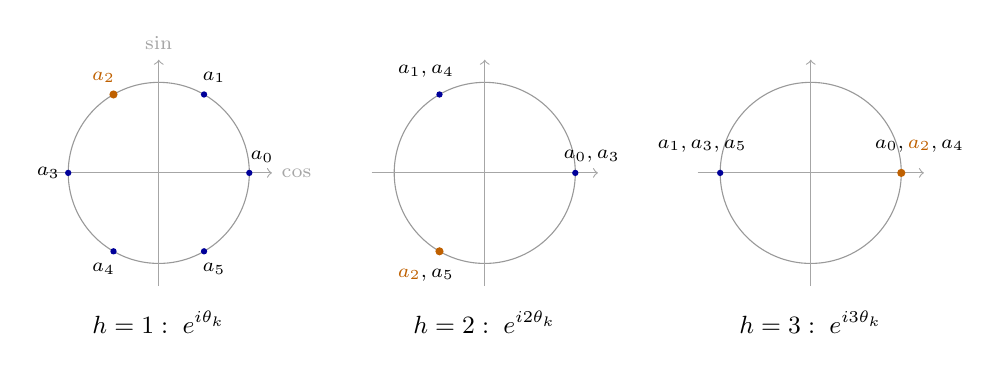
\begin{tikzpicture}[scale=1.15]
    
    \begin{scope}[shift={(0,0)}]
      \draw[black!40] (0,0) circle (1);
      \draw[->,black!35] (-1.25,0)--(1.25,0) node[right,font=\scriptsize]{\(\cos\)};
      \draw[->,black!35] (0,-1.25)--(0,1.25) node[above,font=\scriptsize]{\(\sin\)};
      \foreach \k in {1,3,4,5}{
        \pgfmathsetmacro\ang{60*\k}
      \fill[blue!60!black] (\ang:1) circle (0.035);
      \node[font=\scriptsize] at (\ang:1.22) {\(a_{\k}\)};
    }
    \fill[blue!60!black] (0:1) circle (0.035);
    \node[font=\scriptsize] at (1.14,0.18) {\(a_{0}\)};
    \fill[orange!75!black] (120:1) circle (0.045);
    \node[font=\scriptsize,orange!75!black] at (120:1.22) {\(a_{2}\)};
    \node[font=\small] at (0,-1.65) {\(h=1:\; e^{i\theta_k}\)};
  \end{scope}
  
  \begin{scope}[shift={(3.6,0)}]
    \draw[black!40] (0,0) circle (1);
    \draw[->,black!35] (-1.25,0)--(1.25,0);
    \draw[->,black!35] (0,-1.25)--(0,1.25);
    \fill[blue!60!black] (0:1)   circle (0.035);
    \node[font=\scriptsize] at (1.18,0.18) {\(a_0,a_3\)};
    \fill[blue!60!black] (120:1) circle (0.035);
    \node[font=\scriptsize] at (120:1.3) {\(a_1,a_4\)};
    \fill[orange!75!black] (240:1) circle (0.045);
    \node[font=\scriptsize] at (240:1.3) {\(\textcolor{orange!75!black}{a_2},a_5\)};
    \node[font=\small] at (0,-1.65) {\(h=2:\; e^{i2\theta_k}\)};
  \end{scope}
  
  \begin{scope}[shift={(7.2,0)}]
    \draw[black!40] (0,0) circle (1);
    \draw[->,black!35] (-1.25,0)--(1.25,0);
    \draw[->,black!35] (0,-1.25)--(0,1.25);
    \fill[orange!75!black] (0:1) circle (0.045);
    \node[font=\scriptsize] at (1.2,0.3) {\(a_0,\textcolor{orange!75!black}{a_2},a_4\)};
    \fill[blue!60!black] (180:1) circle (0.035);
    \node[font=\scriptsize] at (-1.2,0.3) {\(a_1,a_3,a_5\)};
    \node[font=\small] at (0,-1.65) {\(h=3:\; e^{i3\theta_k}\)};
  \end{scope}
\end{tikzpicture}
\caption{Cyclic encoding for period \(p=l=6\), at three harmonics.
Coefficient \(a_k\) is encoded at angle \(\theta_k = 2\pi k/p\). Harmonic \(h\) stores the
real and imaginary parts of \(e^{2\pi i\cdot k\cdot h/p}\).
Adjacent coefficients (modulo \(l,m\)) are mapped to adjacent angles. At \(h=1\) the map is one-to-one.
At \(h=2\) the map identifies slots \(k\) and \(k+3\). The harmonics \(h \le \lfloor p/2\rfloor = 3\) form a complete Fourier basis
for functions of position on the period-\(6\) cycle, which is why we chose \(H\geq 3\) for training on \(l=6=m\) codes.}\label{fig:unitcircle}
\end{figure*}

\noindent The encoder architecture is given in Figure~\ref{fig:encoderArchitecture}
\begin{figure*}[htbp]
\centering
\resizebox{\linewidth}{!}{%
\begin{tikzpicture}[archfont, >={Stealth[length=2.2mm]}]

\node[input] (poly) at (0, 0) {polynomial coefficients\\ $[\,a(x)\; a(y)\; b(x)\; b(y)\,]$};
\node[pre] (tok)  at (4.6, 0) {tokenizer + cyclic\\ positional encoding\\ ($H$ harmonics)};
\node[pre] (trf)  at (8.4, 0) {Transformer encoder\\ $d{=}64$, 4 heads\quad $\times\,2$\\ {\footnotesize $\sim$68K parameters}};
\node[pre, text width=17mm] (pool) at (11.7, 0) {attention\\ pooling};

\node[head] (curve) at (16.2,  1.2) {curve head\\ $64{\to}64{\to}5$, sigmoid\\ {\footnotesize $\hat p\in[0,1]^5$ \;($\sim$4.5K)}};
\node[head] (khead) at (16.2, -1.2) {$k$-head\\ $64{\to}64{\to}1$\\ {\footnotesize $\widehat{\log(1{+}k)}$ \;($\sim$4.2K)}};

\draw[arr] (poly) -- (tok);
\draw[arr] (tok) -- coordinate[midway] (m1) (trf);
\draw[arr] (trf) -- coordinate[midway] (m2) (pool);
\draw[arr] (pool.east) -- ++(6mm,0) coordinate[midway] (m3) |- (curve.west);
\draw[arr] (pool.east) -- ++(6mm,0) |- (khead.west);

% Text callouts with diagonal lines, since when I rendered this the text was mushed up together
\node[callout] (c1) at (5.6, 1.9)  {$(2l{+}2m)\times(9{+}2H)$};
\draw[lead] (c1.south) -- (m1);
\node[callout] (c2) at (10.2, 1.9) {$(2l{+}2m)\times 64$};
\draw[lead] (c2.south) -- (m2);
\node[callout] (c3) at (13.1, -1.6) {$64$};
\draw[lead] (c3.north) -- (m3);

% cut line: the task heads are discarded after pretraining
\draw[dashed, black!60, semithick]
  ($(pool.east)+(1mm,2.3)$) -- ($(pool.east)+(1mm,-2.3)$);
\node[font=\large, rotate=-90, text=black!60] at ($(pool.east)+(1mm,2.55)$) {\ding{34}};

\node[anchor=north west, align=left, font=\sffamily\footnotesize, text=black]
  at (0, -2.8)
  {\tikz{\node[pre, text width=4mm, minimum height=3mm, inner sep=1pt]{};}\;
     Encoder carried over into Figure~\ref{fig:hybrid}\qquad
   \tikz{\node[head, text width=4mm, minimum height=3mm, inner sep=1pt]{};}\;
     Pretraining task heads. Discarded (\ding{34}) before carrying into PPO agent.};

\end{tikzpicture}%
}
\caption{The encoder trained in advance by the
multi-task loss of Section~\ref{sec:critic}. A shared trunk feeding a curve
head and a \(k\)-head. The parameters depend only on
\((H, d_{\mathrm{model}}, \text{heads}, \text{layers})\), but not on \((l,m)\), i.e., 
the token count \(2l+2m\) varies with code size, but the token width \(9+2H\) does
not. The two task heads are discarded once training is done. The rest of the network
(blue, \(\sim\)68K parameters at \(H{=}3\)) is carried over to the agent architecture in Figure~\ref{fig:hybrid}.}
\label{fig:encoderArchitecture}
\end{figure*}


\subsection{The logical-qubit features\label{sec:kFeatures}}
Recall from Definition~\ref{def:reward} that if the number of logical qubits \(k\), is below \(k_{\min}\) 
the reward is a deterministic function of \(k\). The environment computes \(k\) by Gaussian elimination over \(GF(2)\) at every step.
It is therefore sensible to help both the agent and the critic to consume \(k\) as an input, and address it immediately. 
Otherwise, we would have to either teach the agent to perform Gaussian elimination, which is somewhat wasteful, or, 
force (by some design insight) to steer towards codes with sufficiently high number of logical qubits. We therefore pass three scalars,
\[
\big[\; \min(k-k_{min},0)/k_{min}, \quad \mathbf{1}_{k \ge k_{min}}, \quad \log(1+k) \;\big],
\]
i.e.:
\begin{enumerate}
\item The (normalised) difference between the minimum number of logical qubits required
\item An indicator of whether the requirement is met, and
\item \(\log(1+k)\)
\end{enumerate} 


\subsection{The fusion layer\label{sec:fusion}}
The three branches are combined by concatenation followed by a single \(\tanh\) layer,
\[
  323 = 64_{\mathrm{enc}} + 256_{\mathrm{mlp}} + 3_{k} \;\longrightarrow\; 256 ,
\]
the output of which is the representation read by the instance head (two instances, one for the critic, one for the actor).

\noindent Fusing the three branches of the architecture later rather than sooner allows us to inspect 
each branch, and potentially hot-plugging branches between trained models, interchanging branches without harming the rest of the network.

\subsection{The policy head and the value head\label{sec:heads}}
The action as we defined it in Section~\ref{sec:mdp} is a tuple \(A^{a(x)},A^{b(x)},A^{a(y)},A^{b(y)}\) of four
per-polynomial actions, each of which flips at most one coefficient. This dictates what the policy head 
should look like. It is made of four independent categorical distributions, one per polynomial, 
of size \(l+1\) for \(a(x),b(x)\) and \(m+1\) for \(a(y),b(y)\), i.e., 
one entry per coefficient, and an additional ``no-op''.
This makes (\(7\) categories each for \(l=m=6\)). 
The four are conditionally independent given the state, 
so the log probability of a joint action is the sum of the four log probabilities. 
%and the entropy bonus decomposes in the same way.
\noindent We point out, that single cells changes of \(H^X,H^Z\) directly, using an independent Bernoulli output per matrix cell, 
the head would have \(\mathcal{O}({(lm)}^{2})\) outputs, quadratic in the code size.
This is a place to state again, that the policy construction benefits from mirroring the code construction, and that otherwise the agent would have to learn
(or otherwise be constrained) to reproduce code qualities, a sampling inefficiency.

\noindent The value head is a single linear map \(256 \to 1\) returning \(\hat V(s)\), trained on the PPO value
target of Algorithm~\ref{alg:main}.
Since the actor and the critic are separate instances of Figure~\ref{fig:hybrid}, 
the value head reads its own trunk, and the two networks share no weights during
PPO even though they may start from the same pretrained encoder. 
The reader should be aware that there is a body of work where the actor and critic share weights, and that we did not explore such 
a path, and leave it as potential further work.


\subsection{Pretraining the encoder\label{sec:critic}}
We now return to the branch of Section~\ref{sec:encoderBranch} and ask:\\
\textit{Can we train the encoder to improve sampling efficiency, and speed up training by guiding the agent to better codes ?}\\

\noindent Unlike the MLP branch, where the input width is a function of the code size, the input of the encoder has code-size-agnostic width.
The encoder maps a code to a latent description of that code.
This could be a supervised problem for which we already have data, i.e., the dataset of
Section~\ref{sec:dataset}, and Appendix~\ref{appendix:dataset}, which contains evaluated codes, each logged with its polynomials, its number
of logical qubits, and its Monte-Carlo error counts.

\noindent We therefore train the encoder in advance as a surrogate model, i.e., from a code's polynomials
\polynomials{} we train it to predicts
\begin{itemize}
      \item The monte-carlo combined error and failure rate curve and
      \item The number of logical qubits \(k\).
\end{itemize}
Which are the two ingredients that make up the reward in Definition~\ref{def:reward}.
These two tasks can be expressed as two terms of a loss function for the encoder, a multi-task sum
\begin{equation}
\begin{split}
  \mathcal{L} \;&=\; \underbrace{\tfrac{1}{5}\sum_{i=1}^{5} n\cdot\mathrm{BCE}\!\big(\hat p_i,\,c_i/n\big)}_{\text{Binomial NLL of the curve}}\\
  \;&+\; \lambda_k\,\underbrace{{\big(\widehat{\log(1+k)}-\log(1+k)\big)}^2}_{\text{\(k\)-head MSE}}
  \end{split}
\end{equation}
\noindent The two heads used here are discarded once pretraining is done, and the rest of the weights are carried over into
Figure~\ref{fig:hybrid} and plugged as the weights of the encoder that produced the \(64\)-dimensional latent representation.

\noindent The motivation behind this was, that a representation which is sufficient to predict how a code performs is also a
good starting point for a critic that has to estimate what the code value is, and for an actor that has to
decide how to improve it.

\noindent This extrapolation was expected to be hard, since for a fixed physical error probability \(p\), 
the probability that a sampled error is trivial is \({(1-3p)}^{N}\), where \(N=2lm\) is the number of physical qubits of a BB code. 
As \(N\) grows, this quantity reduces, and for a fixed number of samples in a monte carlo evaluation (we use \(50\) samples for each \(p\)) 
does not take this into account. In addition to this, a \(6,6\) code can have a maximum number of logical qubits of \(72\), and this number grows with the size of the code.

\noindent Our approach is to train the encoder at small \(l,m\) and then use it unchanged
or cheaply adapt (``ground'') it at larger sizes. The token design explained in Table~\ref{tab:token-features} of
Section~\ref{sec:encoderBranch} makes this possible in principle, i.e., features are
extracted identically at every size. Whether the learned weights actually succeed in extrapolating is a
question which we answer with a sweep over training recipes.
We trained over several \textit{\textbf{training recipes}}, which vary in which values of \((l,m)\in\{(6,6),\,(9,6),\,(12,6),\,(15,3)\}\) are we training on, 
how many harmonics are used \(H\), and which labels, the encoder consumes, as explained below:

\noindent \textbf{(6,6) only} using both labels: the error-rate data and the number of logical qubits \(k\).\\
\noindent\textbf{(6,6) + \(k\)-grounding} Fine-tune the above baseline at the three larger sizes
using the \(k\)-prediction task alone on the larger sizes, not using the error-rate data. Fine tuning is done using 2 epochs and at a lower training rate. The rationale is that \(k\) is
computable exactly at any size by Gaussian elimination over \(GF(2)\), so
this adaptation requires no Monte-Carlo decoder labels at larger sizes. We ground in two
variants, both include \(k\) loss (consuming the \(k\) labels of the bigger codes): \textbf{\textit{anchored}} and \textbf{\textit{non-anchored}}.
In the \textbf{anchored} variant, we revisit the original \(6,6\) curve task while training on new labels, as a guard against forgetting. In the \textbf{non-anchored} we do not revisit the \(6,6\).\\
\noindent\textbf{Mixed sizes} Train on mixed sizes jointly on the full task (curve and \(k\)) using the dataset codes in sizes:
\begin{itemize}
\item \((6,6)\) + \((9,6)\)
\item \((6,6)\) + \((9,6)\) + \((12,6)\)
\item \((6,6)\) + \((9,6)\) + \((12,6)\) + \((15,3)\)
\end{itemize}
\noindent Each recipe, as documented in Table~\ref{tab:recipes}, is trained several times with independent seeds.

\begin{table*}[t]
  \centering
  \caption{Encoder training recipes. Every recipe was trained at each
  \(H \in \{3,4,6,7,10\}\) with ten independent seeds (50 models per recipe,
  300 in total). Grounded models are initialised from the \((6,6)\)-only
  checkpoint with matching \(H\) and seed, so ground-vs-baseline comparisons
  are paired by lineage. Each size's pool is partitioned \(80/10/10\) into
  training, validation and test sets by the model's own seed; ``Training
  codes'' is the training partition summed over the recipe's sizes, and the
  best epoch is selected on the validation partition. Every trained model is
  then evaluated on the full pools of all seven code sizes which include codes that the model has seen.}
  \label{tab:recipes}
  \small
  \begin{tabular}{lllrrcc}
    \toprule
    Recipe &  \makecell{\(k\)\\labels} & \makecell{Curve\\labels}
    & \makecell{Training \\codes} & \makecell{Evaluation\\ codes} & lr & \makecell{Best epoch\\ (val)} \\
    \midrule
    \mixedSixSix                      & \((6,6)\) & \((6,6)\)
      &    716\,040 & 38\,005\,438 & \(10^{-3}\) & 23 [20--23] \\
    \mixedSixSixSixNine                  & \(+(9,6)\) & same as \(k\)
      & 2\,912\,631 & 38\,005\,438 & \(10^{-3}\) & 11 [10--11] \\
    \mixedSixSixSixNineOneTwoSix              & \(+\,(12,6)\) & same as \(k\)
      & 3\,995\,213 & 38\,005\,438 & \(10^{-3}\) & 7 [5--7] \\
    \mixedSixSixSixNineOneTwoSixOneFiveThree          & \(+\,(15,3)\) & same as \(k\)
      & 7\,525\,051 & 38\,005\,438 & \(10^{-3}\) & 5 [4--5] \\
    \midrule
    \groundAnchored &  all four & \((6,6)\) only
      & 7\,525\,051 & 38\,005\,438 & \(10^{-4}\) & 1 [0--1] \\
    \groundPure     &  all four & none
      & 7\,525\,051 & 38\,005\,438 & \(10^{-4}\) & 1 [1--1] \\
    \bottomrule
  \end{tabular}
\end{table*}


\subsubsection{Evaluation (of the encoder)\label{sec:encoderEvaluation}}
\noindent We evaluate each model on the entire dataset, four sizes that were included in the training recipes, and three that were not, 
but using Mean Absolute Error (MAE):\\
\noindent \textbf{\(k\)-MAE} Error of the \(k\)-head in logical qubits. between actual number of logical qubits, shown in Figure~ ref{fig:eval-encoder-kMae}, and \\
\noindent \textbf{Curve-MAE} Per error point MAE of the predicted vs. measured shown in Figure~\ref{fig:point_mae}.\\
\noindent We note that this is not the metric on which training was done. While training was meant to enable transference, we evaluate the resulting models in MAE terms to see if transference was successful.

\noindent Table~\ref{tab:kCurveAlignment} shows a tension between successful prediction on \(k\) vs. the curve. 
By looking at rank correlation, we see that at unseen code sizes there is negative correlation, suggesting the encoder cannot succeed at extrapolating \textbf{both} metrics.
With respect to predicting the curve, Figure~\ref{fig:point_mae} shows the prediction for \(p\in\{0.01,0.0316\}\). As expected, predicting the error rate is harder a larger code sizes, but all models seem to be clustered (in agreement), including their in their collective failure at the \((3,27)\) size at \(p=0.01\) and \(21,18\) at \(p=0.0316\).

\begin{table*}[t]

  \centering
  \caption{Rank correlation between the encoder's \(k\)-MAE and its curve-MAE.
  Rows are training recipes, columns are the code parameters \((l,m)\) the encoder
  was evaluated on. A positive entry means the codes whose \(k\) is predicted well are
  also the codes whose error curve is predicted well. A negative value means the two
  objectives disagree. The three rightmost sizes appear in none of the recipes, so they
  are pure extrapolation. The negative correlations in the last row, where the model was
  trained on the \((6,6)\) codes dataset and grounded using \(k\) labels, as well as in
  the rightmost three columns, suggest there is a tension between predicting \(k\) and
  predicting the performance of a code.}
  \label{tab:kCurveAlignment}
  \footnotesize
  \setlength{\tabcolsep}{8pt}
  \renewcommand{\arraystretch}{1.15}
  \begin{tabular}{@{}l *{4}{S[table-format=-1.2]} @{\hspace{2em}} *{3}{S[table-format=-1.2]}@{}}
    \toprule
    %\multirow{2}{*}{\diagbox[width=7cm,height=2.7\line]{\textbf{Recipe}}{\textbf{Code parameters} \((l,m)\)}}
    & \multicolumn{4}{c}{Sizes named in the recipes}
    & \multicolumn{3}{c}{Unseen sizes} \\
    \cmidrule(lr){2-5} \cmidrule(l){6-8}
    & {\((6,6)\)} & {\((9,6)\)} & {\((12,6)\)} & {\((15,3)\)}
    & {\((5,15)\)} & {\((3,27)\)} & {\((21,18)\)} \\
    \midrule
    \texttt{\mixedSixSix}                     &  0.36 &  0.21 & -0.05 &  0.22 & -0.46 & -0.50 & -0.10 \\
    \texttt{\mixedSixSixSixNine}                  &  0.29 &  0.47 & -0.05 &  0.39 &  0.17 & -0.62 &  0.56 \\
    \texttt{\mixedSixSixSixNineOneTwoSix}              & -0.03 &  0.61 &  0.76 &  0.70 & -0.19 & -0.39 &  0.40 \\
    \texttt{\mixedSixSixSixNineOneTwoSixOneFiveThree}          &  0.03 &  0.12 &  0.34 &  0.39 & -0.53 & -0.40 &  0.06 \\
    \addlinespace
    \texttt{\groundAnchored} &  0.42 &  0.08 &  0.07 & -0.15 & -0.21 & -0.35 & -0.26 \\
    \texttt{\groundPure}     &  0.34 & -0.03 &  0.00 & -0.08 & -0.12 & -0.43 & -0.23 \\
    \bottomrule
  \end{tabular}
\end{table*}


% \begin{table}[t]
%   \centering
%   \caption{Each of the 300 encoders is evaluated on all
%   seven sizes. ``In recipes'' marks the four sizes that appear in at least one
%   training recipe. The table counts records that are distinct polynomials (recall that this does not imply different codes) on the \texttt{geometric5} error range.}
%   \label{tab:evaluationPools}
%   \begin{tabular}{lrrc}
%     \toprule
%     \((l,m)\) & \(n=2lm\) & Codes & In recipes \\
%     \midrule
%     \((6,6)\)   &  72 &    895\,050 & \checkmark \\
%     \((15,3)\)  &  90 &  4\,412\,297 & \checkmark \\
%     \((9,6)\)   & 108 &  2\,745\,740 & \checkmark \\
%     \((12,6)\)  & 144 &  1\,353\,227 & \checkmark \\
%     \((5,15)\)  & 150 & 18\,402\,947 & \\
%     \((3,27)\)  & 162 & 10\,148\,123 & \\
%     \((21,18)\) & 756 &     48\,054 & \\
%     \midrule
%     Total       &     & 38\,005\,438 & \\
%     \bottomrule
%   \end{tabular}
% \end{table}


\begin{figure*}[htbp]
    \centering
    \begin{subfigure}{0.49\linewidth}
        \centering
        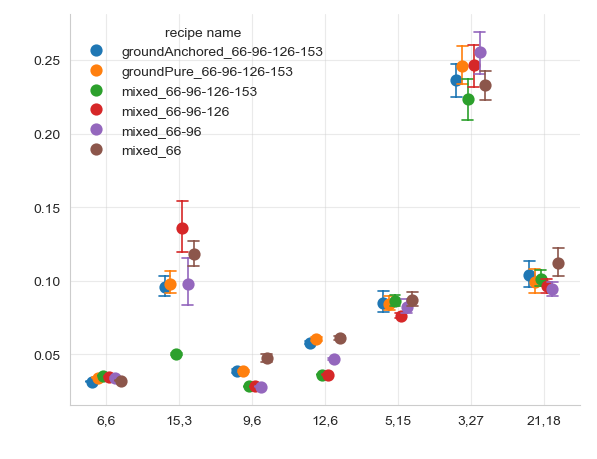
\includegraphics[width=\linewidth]{art/encoder/error_point_prediction_for_point_2_mae_per_code_size.png}
    \end{subfigure}
    \hfill
    \begin{subfigure}{0.49\linewidth}
        \centering
        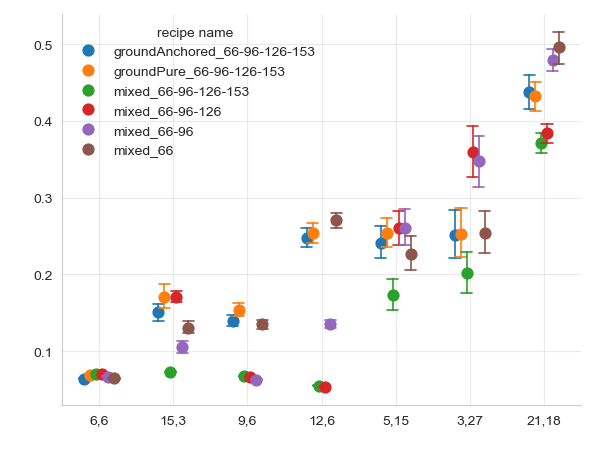
\includegraphics[width=\linewidth]{art/encoder/error_point_prediction_for_point_3_mae_per_code_size.png}
    \end{subfigure}
    \caption{Mean absolute error of prediction vs. measured logical error rate across the \(300\) encoders trained, plotted for \(p\in\{0.01, 0.0316\}\).\label{fig:point_mae}}
\end{figure*}

